\begin{multicols}{3}
\begin{textbox}{Neural Networks}
\begin{subbox}{subbox}{ Introduction}
\scriptsize
Now it’s time for you to create your first neural network using PyTorch. This section will walk you through the process of:
\begin{itemize}
    \item 
Creating a simple neural network model
    \item Training the network
    \item Visualizing the results of the network
    \item Tweaking the network
\end{itemize}
\end{subbox}
\begin{subbox}{subbox}{ Data }
\scriptsize

First we need some sample data to train our network on. The example dataset consists of 2D points along two interleaving half circles, figure below. 

\centering
\includegraphics[scale=0.3]{Figures/NN/NNFigure1.png}

\end{subbox}
%%%%% Create a Simple Neural Network
\begin{subbox}{subbox}{ Create a Simple Neural Network}
\scriptsize
For this example we want to have a simple neural network consisting of 3 layers:

\begin{itemize}
\item
 input layer of size 2 (our points have 2 coordinates)
\item hidden layer of size 16 (you can play with different numbers here)

 \item
 output layer of size 2 (we want the have the scores for the two classes)
 \end{itemize}
 
During the course you will deal with different kinds of neural networks.
\end{subbox}
\end{textbox}
%%%%%%%%%%%%
\begin{textbox}{Create a Simple Neural Network}
\begin{subbox}{subbox}{Programing the Network }
\scriptsize


PyTorch provides a base class for all neural network modules called nn.Module. You need to inherit from nn.Module and implement some important methods:

\begin{itemize}
    \item[
\textbf{init}]
In the \textbf{init} method you need to define the structure of your network. Here you will specify what layers will the network consist of, what activation functions will be used etc.
\item[\textbf{forward}]
All neural network modules need to implement the \textbf{forward} method. It specifies the computations the network needs to do when data is passed through it.
\item[\textbf{predict}]
This is not an obligatory method of a neural network module, but it is a good practice if you want to quickly get the most likely label from the network. It calls the forward method and chooses the label with the highest score.
\item[\textbf{train}]
This is also not an obligatory method, but it is a good practice to have. The method will be used to train the network parameters and will be implemented later in the notebook.
\end{itemize}

\end{subbox}
\begin{subbox}{subbox}{Example Architecture the Network }
\scriptsize
The schematic below shows an example neural network with two nodes in the input layers, four nodes in the hidden layer (in the code there are 16 nodes) and two nodes in the output layer. 
% NEURAL NETWORK no text
\begin{center}
\begin{tikzpicture}[x=2.2cm,y=1.4cm]
  \message{^^JNeural network without text}
  \readlist\Nnod{2,4,2} % array of number of nodes per layer
  
  \message{^^J  Layer}
  \foreachitem \N \in \Nnod{ % loop over layers
    \def\lay{\Ncnt} % alias of index of current layer
    \pgfmathsetmacro\prev{int(\Ncnt-1)} % number of previous layer
    \message{\lay,}
    \foreach \i [evaluate={\y=\N/2-\i; \x=\lay; \n=\nstyle;}] in {1,...,\N}{ % loop over nodes
      
      % NODES
      \node[node \n] (N\lay-\i) at (\x,\y) {};
      
      % CONNECTIONS
      \ifnum\lay>1 % connect to previous layer
        \foreach \j in {1,...,\Nnod[\prev]}{ % loop over nodes in previous layer
          \draw[connect,white,line width=1.2] (N\prev-\j) -- (N\lay-\i);
          \draw[connect] (N\prev-\j) -- (N\lay-\i);
          %\draw[connect] (N\prev-\j.0) -- (N\lay-\i.180); % connect to left
        }
      \fi % else: nothing to connect first layer
      
    }
  }
  
  % LABELS
  \node[above=5,align=center,mygreen!60!black] at (N1-1.90) {input\\[-0.2em]layer};
  \node[above=2,align=center,myblue!60!black] at (N2-1.90) {hidden layer};
  \node[above=10,align=center,myred!60!black] at (N\Nnodlen-1.90) {output\\[-0.2em]layer};
  
\end{tikzpicture}
\end{center}
\end{subbox}
\end{textbox}
\begin{textbox}{Simple Neural Network in python}
\tiny
\begin{lstlisting}[language=Python]
# Inherit from nn.Module - the base class for neural network modules provided by Pytorch
class NaiveNet(nn.Module):
  """
  NaiveNet architecture
  Structure is as follows:
  Linear Layer (2, 16) -> ReLU activation -> Linear Layer (16, 2)
  """
  \end{lstlisting}
\begin{subbox}{subbox}{\textbf{init} function }
\begin{lstlisting}[language=Python]
  # Define the structure of your network
  def __init__(self):
    """
    Defines the NaiveNet structure by initialising following attributes nn.Linear (2, 16):  Transformation from the input to the hidden layer nn.ReLU: Activation function (ReLU) is a non-linearity which is widely used because it reduces computation.
    The function returns 0 if it receives any negative input, but for any positive value x, it returns that value back. 
    nn.Linear (16, 2): Transformation from the hidden to the output layer   
    Args:
      None
    Returns:
      Nothing
    """
    super(NaiveNet, self).__init__()
    # The network is defined as a sequence of operations
    self.layers = nn.Sequential(
        nn.Linear(2, 16),
        nn.ReLU(),
        nn.Linear(16, 2),
    )
\end{lstlisting}
\end{subbox}
\end{textbox}
\begin{textbox}{Simple Neural Network in python}
\tiny
\begin{subbox}{subbox}{\textbf{forward} function }
\begin{lstlisting}[language=Python]
  # Specify the computations performed on the data
  def forward(self, x):
    """
    Defines the forward pass through the above defined structure
    Args:
      x: torch.Tensor
        Input tensor of size ([3])
    Returns:
      layers: nn.module
        Initialised Layers in order to re-use the same layer for each forward pass of data you make.
    """
    # Pass the data through the layers
    return self.layers(x)
\end{lstlisting}
\end{subbox}
\begin{subbox}{subbox}{\textbf{predict} function }
\begin{lstlisting}[language=Python]
  # Choose the most likely label predicted by the network
  def predict(self, x):
    """
    Performs the prediction task of the network
    Args:
      x: torch.Tensor
        Input tensor of size ([3])
    Returns:
      Most likely class i.e., Label with the highest score
    """
    # Pass the data through the networks
    output = self.forward(x)
    # Choose the label with the highest score
    return torch.argmax(output, 1)
\end{lstlisting}
\end{subbox}

\begin{subbox}{subbox}{\textbf{train} function }
\tiny
\begin{lstlisting}[language=Python]
  # Train the neural network (will be implemented later)
  def train(self, X, y):
    """
    Training the Neural Network
    Args:
      X: torch.Tensor (Input data)
      y: torch.Tensor
        Class Labels/Targets
    Returns:
      Nothing
    """
    pass
\end{lstlisting}
\end{subbox}

\end{textbox}
%%%%%%%%%%%%%%%%%%%%%%%%%%%%%%%%%%%%%%%%%%%%%%%%%%
%%%%%%%%%%%%%%%%%%%%%%%%%%%%%%%%%%%%%%%%%%%%%%%%%%
\begin{textbox}{Train Your Neural Network}
\begin{subbox}{subbox}{Train the Network}
\scriptsize
Now it is time to train your network on your dataset. Don’t worry if you don’t fully understand everything yet - we will cover training in much more details in the next days. For now, the goal is just to see your network in action!

You will usually implement the train method directly when implementing your class NaiveNet. Here, we will implement it as a function outside of the class in order to have it in a separate cell. 
\begin{lstlisting}[language=Python]
# Implement the train function given a training dataset X and corresponding labels y
def train(model, X, y):
  """
    Training the Neural Network
    Args:
      X: torch.Tensor
        Input data
      y: torch.Tensor
        Class Labels/Targets
    Returns:
      losses: Float
        Cross Entropy Loss; Cross-entropy builds upon the idea of entropy from information theory and calculates the number of bits required to represent or transmit an average event from one distribution compared to another distribution.
    """
  # The Cross Entropy Loss is suitable for classification problems
  loss_function = nn.CrossEntropyLoss()
  # Create an optimizer (Stochastic Gradient Descent) that will be used to train the network
  learning_rate = 1e-2
  optimizer = torch.optim.SGD(model.parameters(), lr=learning_rate)
  # Number of epochs
  epochs = 15000
  # List of losses for visualization
  losses = []
  for i in range(epochs):
    # Pass the data through the network and compute the loss
    y_logits = model.forward(X)
    loss = loss_function(y_logits, y)
    # Clear the previous gradients and compute the new ones
    optimizer.zero_grad()
    loss.backward()
    # Adapt the weights of the network
    optimizer.step()
    # Store the loss
    losses.append(loss.item())
  return losses
# Create a new network instance a train it
model = NaiveNet().to(DEVICE)
losses = train(model, X, y)
\end{lstlisting}
\end{subbox}
\end{textbox}
%%%%%%%%%%%%%%%%%%%%%%%%%%%%%%%%%%%%%%%%%%%%%%%%%%
%%%%%%%%%%%%%%%%%%%%%%%%%%%%%%%%%%%%%%%%%%%%%%%%%%
%%%%%%%%%%%%%%%%%%%%%%%%%%%%%%%%%%%%%%%%%%%%%%%%%%
%%%%%%%%%%%%%%%%%%%%%%%%%%%%%%%%%%%%%%%%%%%%%%%%%%
\begin{textbox}{Trained Neural Network}
\begin{subbox}{subbox}{The output of the Neural Network}
\scriptsize
The plot below shows the categorisation boundary for the neural network after learning for the two data types (white and black). The neural network does a reasonable job of separating the data.
\begin{center}
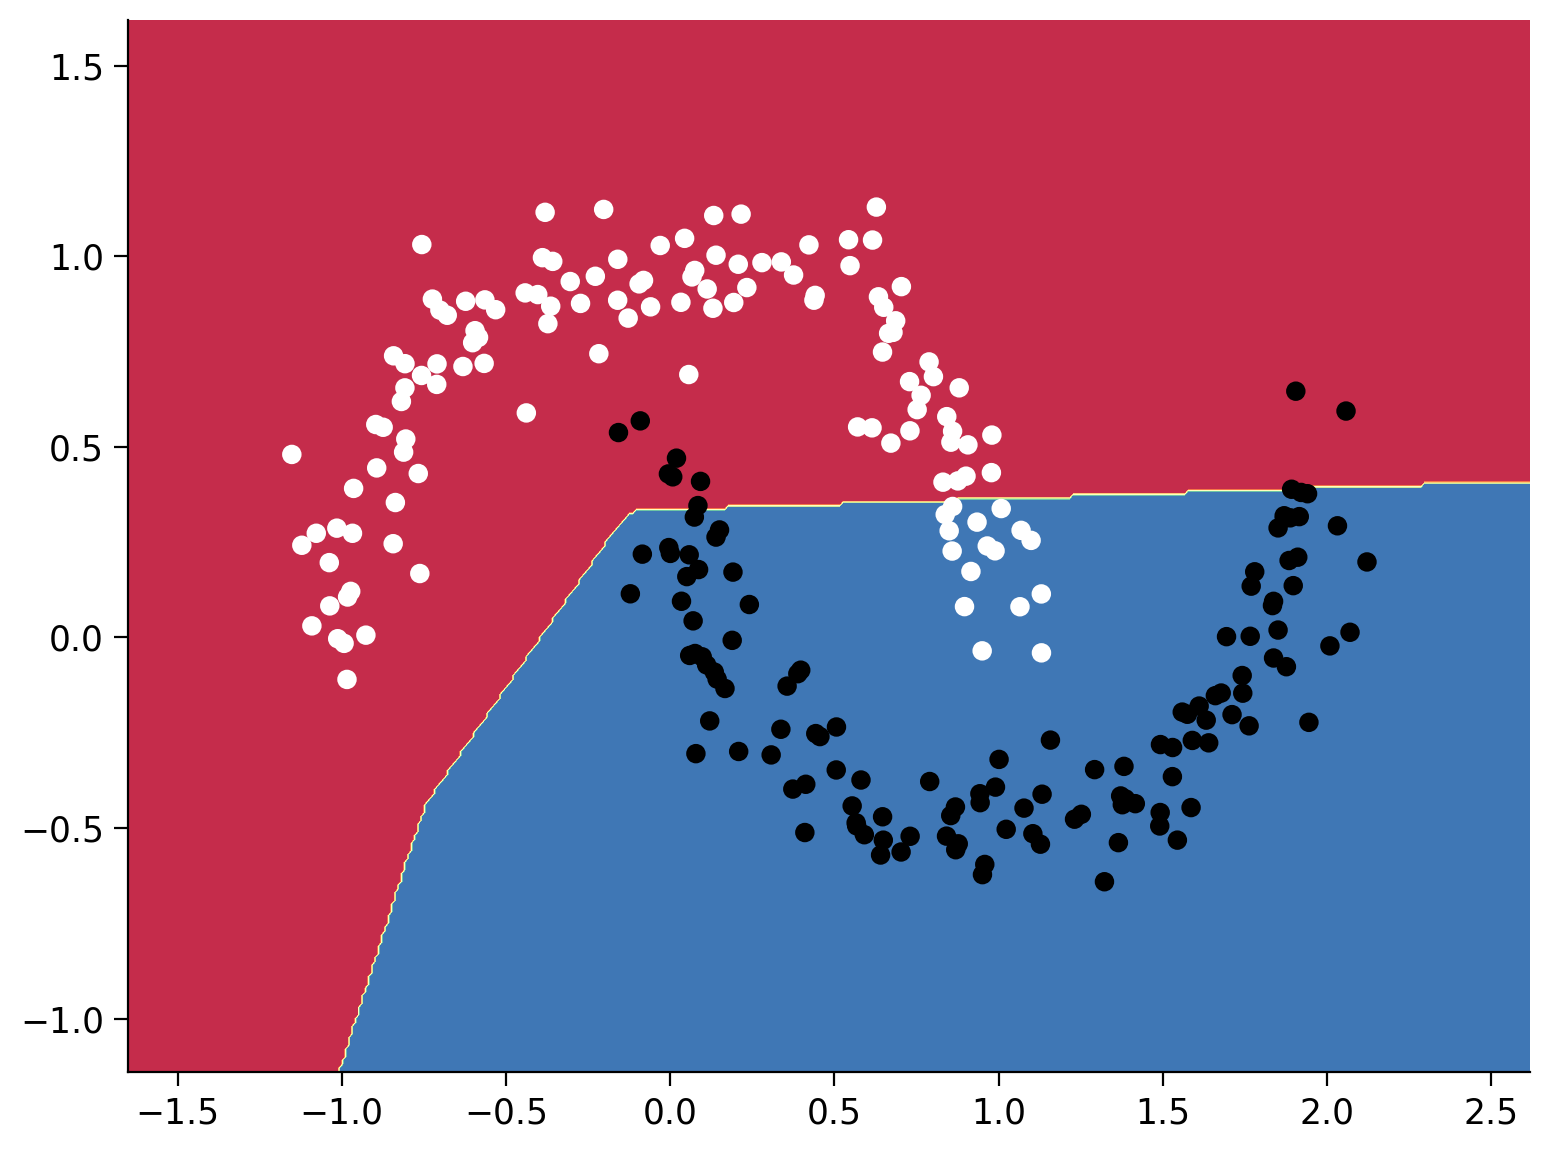
\includegraphics[scale=0.28]{Figures/NN/W1D1_Tutorial1_Learnt.png}
\end{center}
The plot below shows the loss during the training to see how it reduces and converges.
\begin{center}
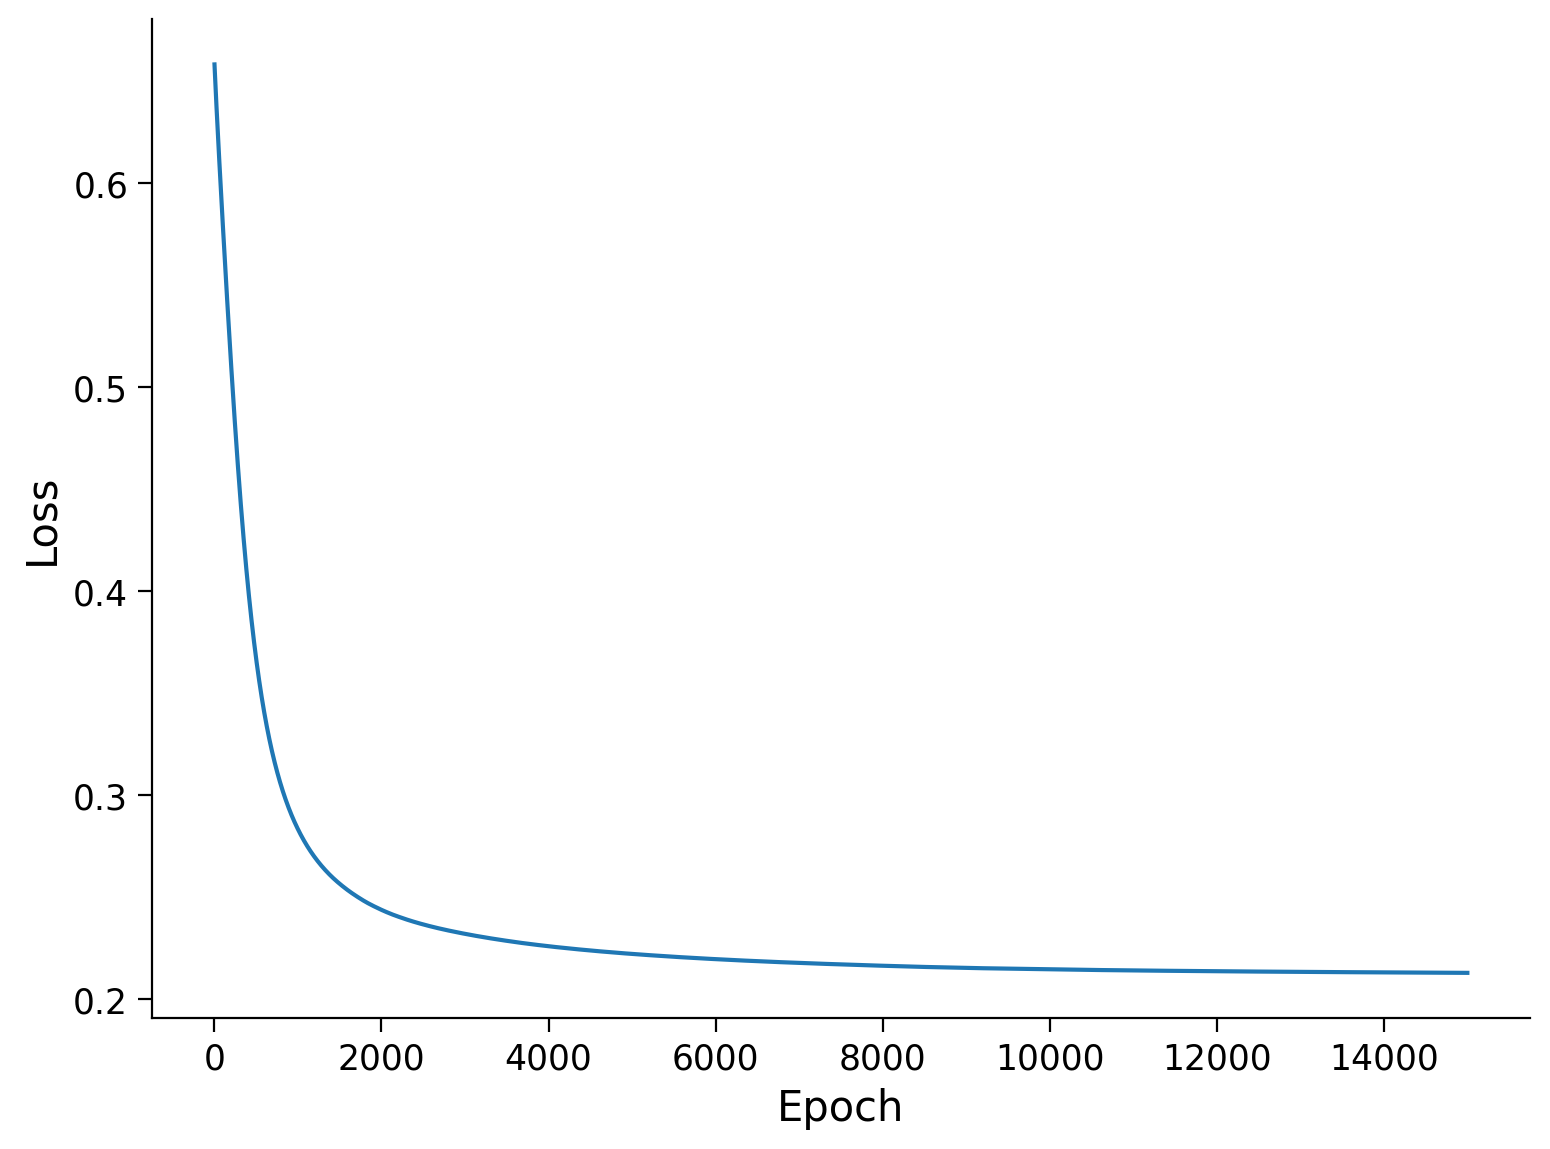
\includegraphics[scale=0.28]{Figures/NN/W1D1_Tutorial1_181_LossFunction.png}
\end{center}

\end{subbox}
\begin{subbox}{subbox}{Tweak your Network}
\scriptsize
You can now play around with the network a little bit to get a feeling of what different parameters are doing. Here are some ideas what you could try:
\begin{itemize}
    \item 
Increase or decrease the number of epochs for training
\item Increase or decrease the size of the hidden layer
\item Add one additional hidden layer
\end{itemize}
Can you get the network to better fit the data?

\end{subbox}
\begin{subbox}{subbox}{W1D1 MusicMatch \musEighth}
\scriptsize
The  
 musical matching for the
 tutorials Basics And Pytorch  is
“Rolling in the Deep” by Adele. 

\end{subbox}
\end{textbox}

%%%%%% APPENDIX
\begin{textbox}{Appendix}
\begin{subbox}{subbox}{ Official PyTorch resources:}
\scriptsize
\begin{itemize}
    \item 
\href{https://pytorch.org/tutorials/}{Pytorch Tutorials}

\item 
\href{https://pytorch.org/docs/stable/tensors.html}{Documentation}

\item  
\href{https://pytorch.org/docs/stable/generated/torch.Tensor.view.html#torch.Tensor.view}{TORCH.TENSOR.VIEW}

\item  
\href{https://pytorch.org/vision/stable/datasets.html}{pre-loaded image datasets}

\end{itemize} 
\end{subbox}
\begin{subbox}{subbox}{ Google Colab Resources:}
\begin{itemize}
    \item 
    \href{https://research.google.com/colaboratory/faq.html}{FAQ including guidance on GPU usage}

 \end{itemize}
\end{subbox}
\begin{subbox}{subbox}{ Books for reference:}
\begin{itemize}
    \item 
    \href{https://www.deeplearningbook.org/}{Deep Learning by Ian Goodfellow, Yoshua Bengio and Aaron Courville}

 \end{itemize}
\end{subbox}
\end{textbox}
\end{multicols}